\begin{figure}[t]
   \centering
   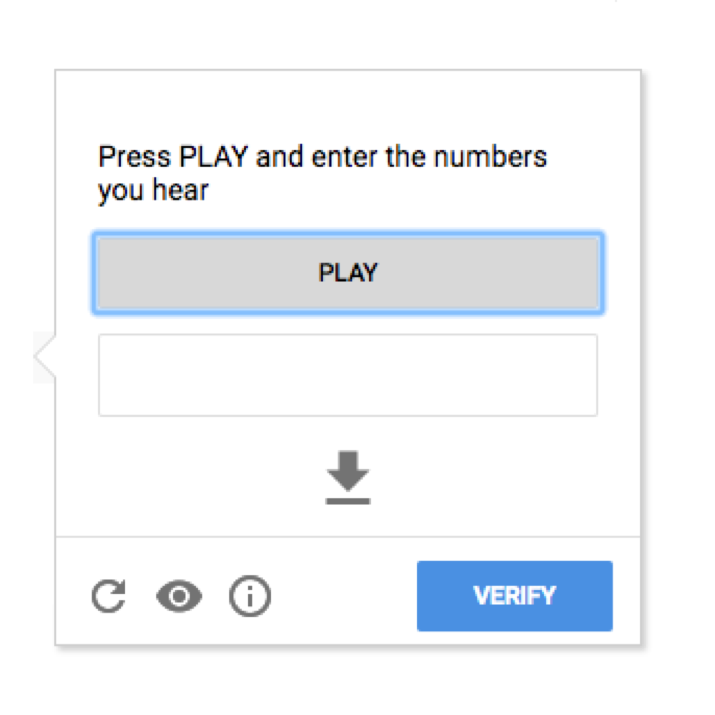
\includegraphics[width=\columnwidth]{figures/Picture1.png}.
   \caption{The ReCAPTCHA widget: Users can play the audio, download the file or request for a new challenge.}
   \label{fig:recaptcha}
\end{figure}

\section{System Overview}
\label{sec:design}

\subsection{Generic System}\mbox{} \
\label{sec:generic}

Our system consists of a crawler that loads the required page, finds the audio element in the page and downloads it. It then converts the audio file into the required audio format and hands it over to another system that connects to the speech recognition web services. Once the transcript is obtained from the service, it hands over the result to the first system that fills the CAPTCHA response and submits the form/challenge.\newline

To build the crawler, we used a Python script with Selenium and ChromeDriver. The script recursively loads the URL that has been hard coded into the system and with Selenium, we fire up the ChromeDriver. Selenium helps in finding the required elements on the page and manipulate them. Once it finds the audio element on the page, it is downloaded and if the file is in MP3 format, we use the Pydub library to convert the file to WAV/FLAC format. We did this as IBM Watson's Speech to Text API expects only a WAV file and Google Speech API expects a FLAC file. These two files are stored with the timestamp of when the first file was initially downloaded.\newline

Next, the control is transferred to the solver script. We implemented this in Node.JS and we used the Naked library available for Python to execute a JavaScript file. The Node.JS script is fired up that takes the converted file and sends it to the appropriate solver using its API and gets back the response. In the case when the solver gives a list of alternative transcriptions for each recognized sound, we select the most appropriate one among them.\newline

We did not require transferring control to the Node.JS module for the Google solvers as we used the Python implementations of Google Speech API.To achieve this, we used the Google Speech API Client module that is available to install via the "pip" command for Python and setting up the credentials via a JSON file that can be downloaded by registering for a new application with the Google Cloud platform. \newline

The script then builds the response based on this and sends it back to the Python script. It then enters the response into the response box using Selenium, and the challenge is submitted. Once it is submitted, we look for some element on the page that is generated which tells the user if the submitted response was correct or not. We again crawl the page for this element and gather this result. We next store these results in a CSV file along with the file name for each challenge we solve. \newline

\subsection{Tweaking for ReCAPTCHA}
\label{sec:recaptcha}

We found that ReCAPTCHA had implemented rate limitation (we talk about this in detail in the forthcoming section). To overcome this limitation, we had to tweak our script to generate random user agent strings that would allow us to bypass the limit. It also generated the audio in MP3 format that had to be converted into WAV. \newline

\subsection{Tweaking for Captchas.net and Telerik}
\label{sec:captchasnet}

Captchas.net and Telerik CAPTCHAs spell out NATO characters and expect the users to solve the challenge using English alphabets. To achieve this, we had to modify our script to map the NATO responses to English alphabets. \newline

\subsection{Tweaking for Live.com}
\label{sec:captchasnet}

As we would have created spam accounts on Live.com in order to verify to evaluate our attack, we preferred not to flood their system with fake accounts. Thus, we modified our system to only crawl and download 100 audio challenges that we manually transcribed and then used the 5 solvers on that dataset to verify with the truth set that we had created. \newline

\subsection{Tweaking for Apple}
\label{sec:captchasnet}

As we did not get the audio file from Apple's CAPTCHA directly, we had to modify our script to open the chrome://media-internals URL simultaneously to grab the playing audio. We also had to send null values to the response box and vary the time delay between the various input fields to mimic a human. \newline

\begin{lstlisting}[caption={Setting Expected Phrases in Google Speech API for Captchas.net solver}]

'speechContext': {

	"phrases": ["Alfa", "Bravo", "Charlie", "Delta", "Echo", "Foxtrot", "Golf", "Hotel", "India", "Juliett", "Kilo", "Lima", "Mike", "November", "Oscar", "Papa", "Quebec", "Romeo", "Sierra", "Tango", "Uniform", "Victor", "Whiskey", "X-ray", "Yankee", "Zulu"
	]

}
\end{lstlisting}
